\documentclass[a4paper,10pt]{article}

\usepackage{graphicx}
\usepackage{float}

% Custom margins setup
\usepackage[left=2cm, right=2cm, top=2cm, bottom=2cm]{geometry}

% Using fontspec for font management
\usepackage{fontspec}
\usepackage[utf8]{inputenc}
\usepackage{minted}
\setmainfont{STIX Two Text}

% Package for creating landscape pages within a document
\usepackage{pdflscape}

\begin{document}

\tableofcontents

\section{Introduction}

This document describes the requirements and modelling of \emph{Wigvana}---an e-commerce platform for buying and selling human hair extensions.

\section{Stakeholders}

\begin{enumerate}
    \item Primary stakeholders:
          \begin{enumerate}
              \item Buyers / Customers:
                    \begin{itemize}
                        \item \textbf{Role}: Individuals or groups purchasing hair extension items.
                        \item \textbf{Interests}: Wide selection, fair prices, accurate product descriptions and images, easy navigation and search, secure payment options, reliable and timely shipping, hassle-free returns/exchanges, good customer service, trend information, personalization.
                    \end{itemize}
              \item Sellers / Vendors / Brands:
                    \begin{itemize}
                        \item \textbf{Role}: Individuals, small businesses, or established brands listing and selling their products on the platform.
                        \item \textbf{Interests}: Access to a large customer base, easy-to-use tools for listing products and managing inventory, fair commission/fee structure, timely payments, reliable platform performance, seller support, marketing opportunities, brand visibility, protection against fraud.
                    \end{itemize}
              \item Platform Owner / Operator (Wigvana):
                    \begin{itemize}
                        \item \textbf{Role}: The entity that builds, manages, and operates the e-commerce platform.
                        \item \textbf{Interests}: Profitability (through commissions, listing fees, advertising, etc.), user growth (both buyers and sellers), platform stability and performance, brand reputation, operational efficiency, legal compliance, competitive advantage, data insights.
                    \end{itemize}
              \item Payment Gateway Providers:
                    \begin{itemize}
                        \item \textbf{Role}: Third-party services facilitating secure online transactions (e.g., Stripe, PayPal, local mobile money operators).
                        \item \textbf{Interests}: Transaction volume, seamless integration, platform reliability, security compliance, timely settlement of funds.
                    \end{itemize}
          \end{enumerate}
    \item Secondary stakeholders:
          \begin{enumerate}
              \item Payment Processors (e.g., Stripe, PayPal, Banks): Facilitate secure transactions.

              \item Logistics \& Shipping Partners (e.g., FedEx, DHL, local couriers): Handle order fulfillment and delivery.

              \item Marketing \& Advertising Partners: Agencies or platforms (Google Ads, Meta) helping attract buyers.

              \item Third-Party Integrations (e.g., CRM, analytics tools): Services enhancing platform functionality.
          \end{enumerate}
\end{enumerate}

\section{Actors}

\subsection{Buyers (Customers)}

The buying actor can behave in two ways:

\begin{itemize}
    \item With their identity established, i.e., \emph{authenticated}.
    \item Browsing without an established identity (Anonymous).
\end{itemize}


Goals:

\begin{enumerate}
    \item Browse/search for fashion products by using:
          \begin{itemize}
              \item Selecting a product functionality:
                    \begin{enumerate}
                        \item Category
                        \item Price
                        \item Search terms
                    \end{enumerate}
              \item Viewing details on a product:
                    \begin{enumerate}
                        \item Name
                        \item Description
                        \item Price
                        \item Images
                        \item Seller details
                    \end{enumerate}
          \end{itemize}


    \item Compare prices, styles, and reviews.

    \item Add items to cart/wishlist.

    \item Make secure payments.

    \item Track orders \& request returns/refunds (Line of communication with vendors).

    \item Leave reviews \& ratings.
\end{enumerate}

\subsection{Sellers (Merchants/Vendors)}

Goals:


\begin{enumerate}
    \item Register \& set up seller profiles.

    \item List, update, and manage product inventory.

    \item Set pricing, discounts, and promotions.

    \item Process \& fulfill orders.

    \item Handle returns/refunds.

    \item Analyze sales performance.
\end{enumerate}

\subsection{Platform Administrator}

Goals:

\begin{enumerate}
    \item Manage user accounts (buyers \& sellers).

    \item Moderate listings (fraud, counterfeit detection).

    \item Handle disputes (refunds, scams).

    \item Monitor platform performance \& security.

    \item Update platform features \& policies.
\end{enumerate}

\section{Use cases}

\begin{itemize}
    \item Search for a product.
    \item Place an order.
\end{itemize}




% \begin{landscape}
%     \section{Landscape Section}
%     This section is rendered in landscape orientation.
% \end{landscape}

\section{Authentication}

\subsection{Authentication flows}
\begin{enumerate}
    \item Login flow
          \begin{figure}[H]
              \centering
              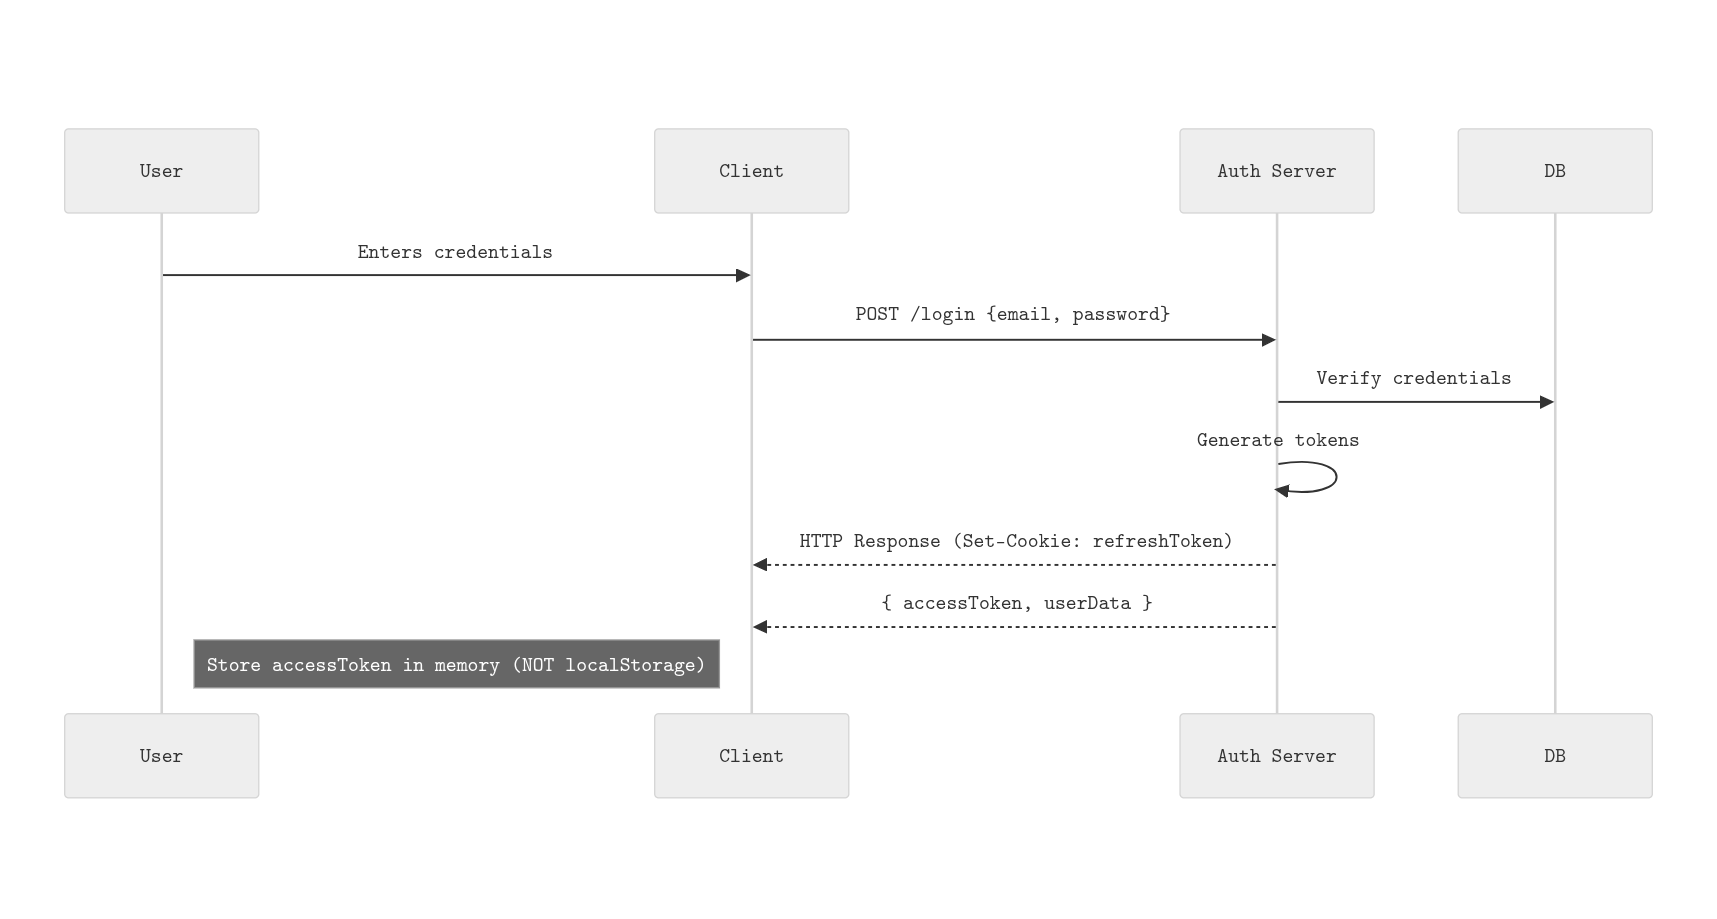
\includegraphics[width=\textwidth]{images/login-flow.png}
              \caption{Login flow.}
              \label{fig:login_flow}
          \end{figure}

          What happens:
          \begin{itemize}
              \item Server validate credentials.
              \item Generates:
                    \begin{enumerate}
                        \item Short-lived access tokens (e.g., 15-30 mins)
                              \begin{minted}[linenos,breaklines]{json}
{
  "sub": "user123",
  "roles": ["user"],
  "iat": 1620000000,
  "exp": 1620001800
}
                                
                                \end{minted}
                        \item Long lived refresh tokens (e.g., 7 days) stored in \texttt{HTTPOnly} cookie.
                    \end{enumerate}
              \item Client stores access token in memory (React/Vue state, Angular service)
          \end{itemize}
    \item Accessing protected resources.
          \begin{figure}[H]
              \centering
              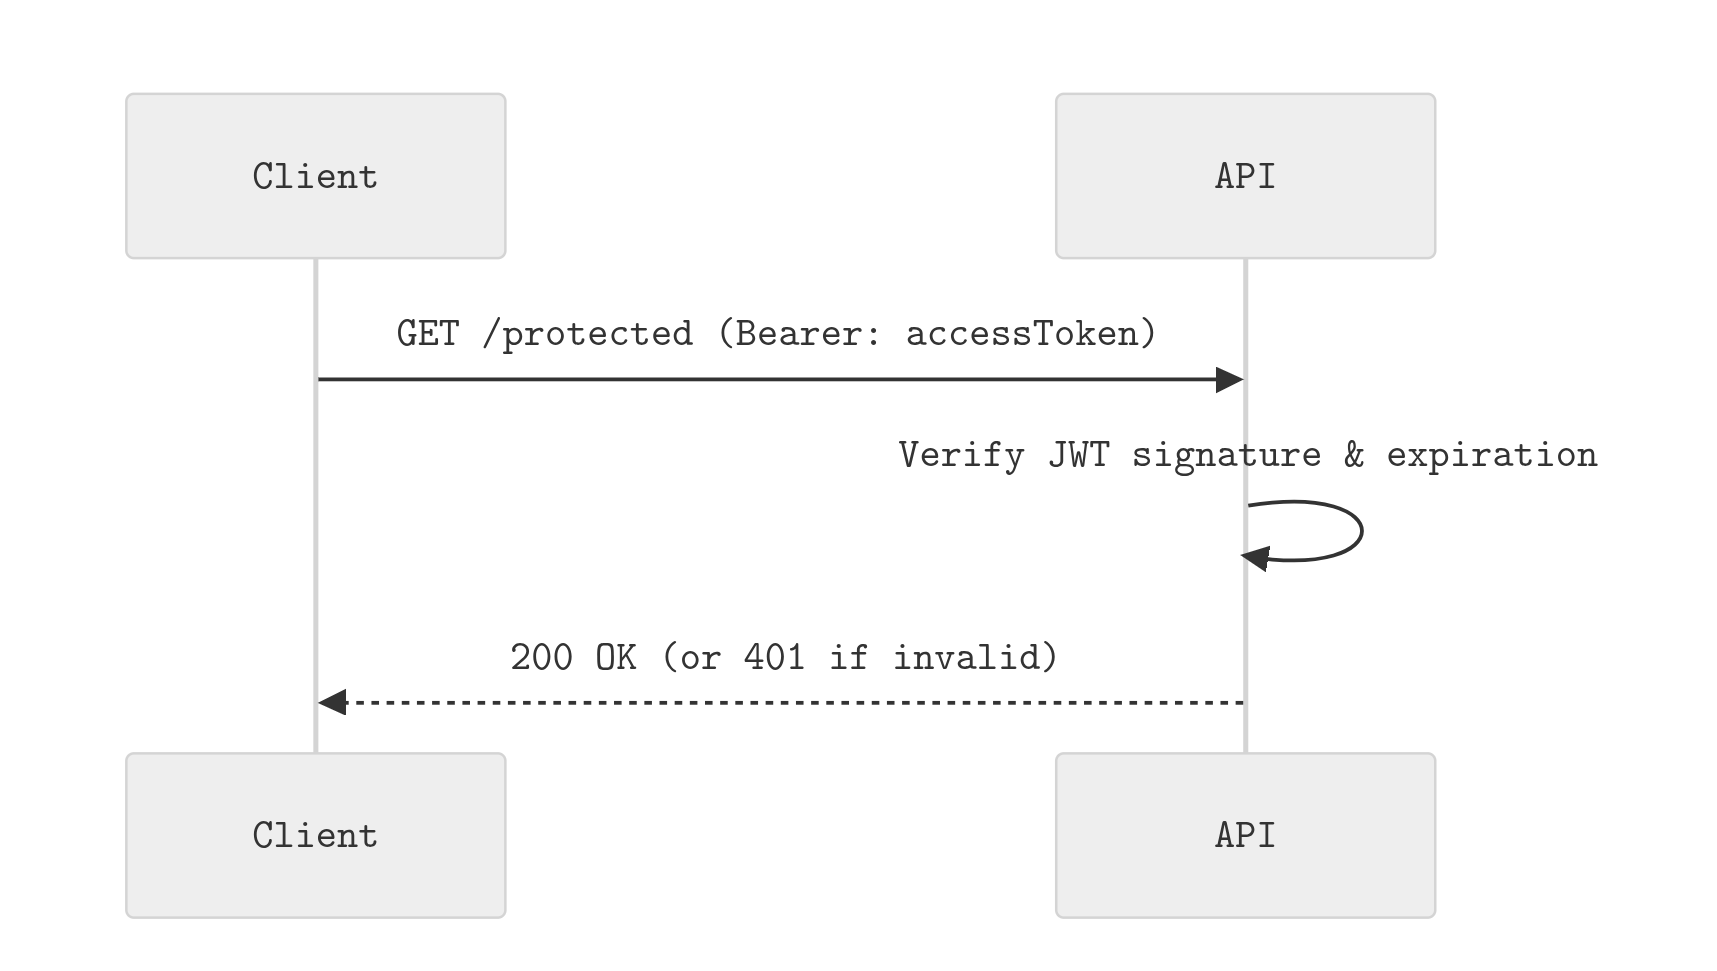
\includegraphics[width=\textwidth]{images/protected.png}
              \caption{Protected resource access.}
              \label{fig:procted_access}
          \end{figure}

          What happens:

          \begin{itemize}
              \item Validate JWT signature using server's secret/public key.
              \item Check \texttt{exp} claim.
              \item Verify token wasn't revoked (optional denylist for critical systems)
          \end{itemize}
    \item Access token expiration (silent refresh)
          \begin{figure}[H]
              \centering
              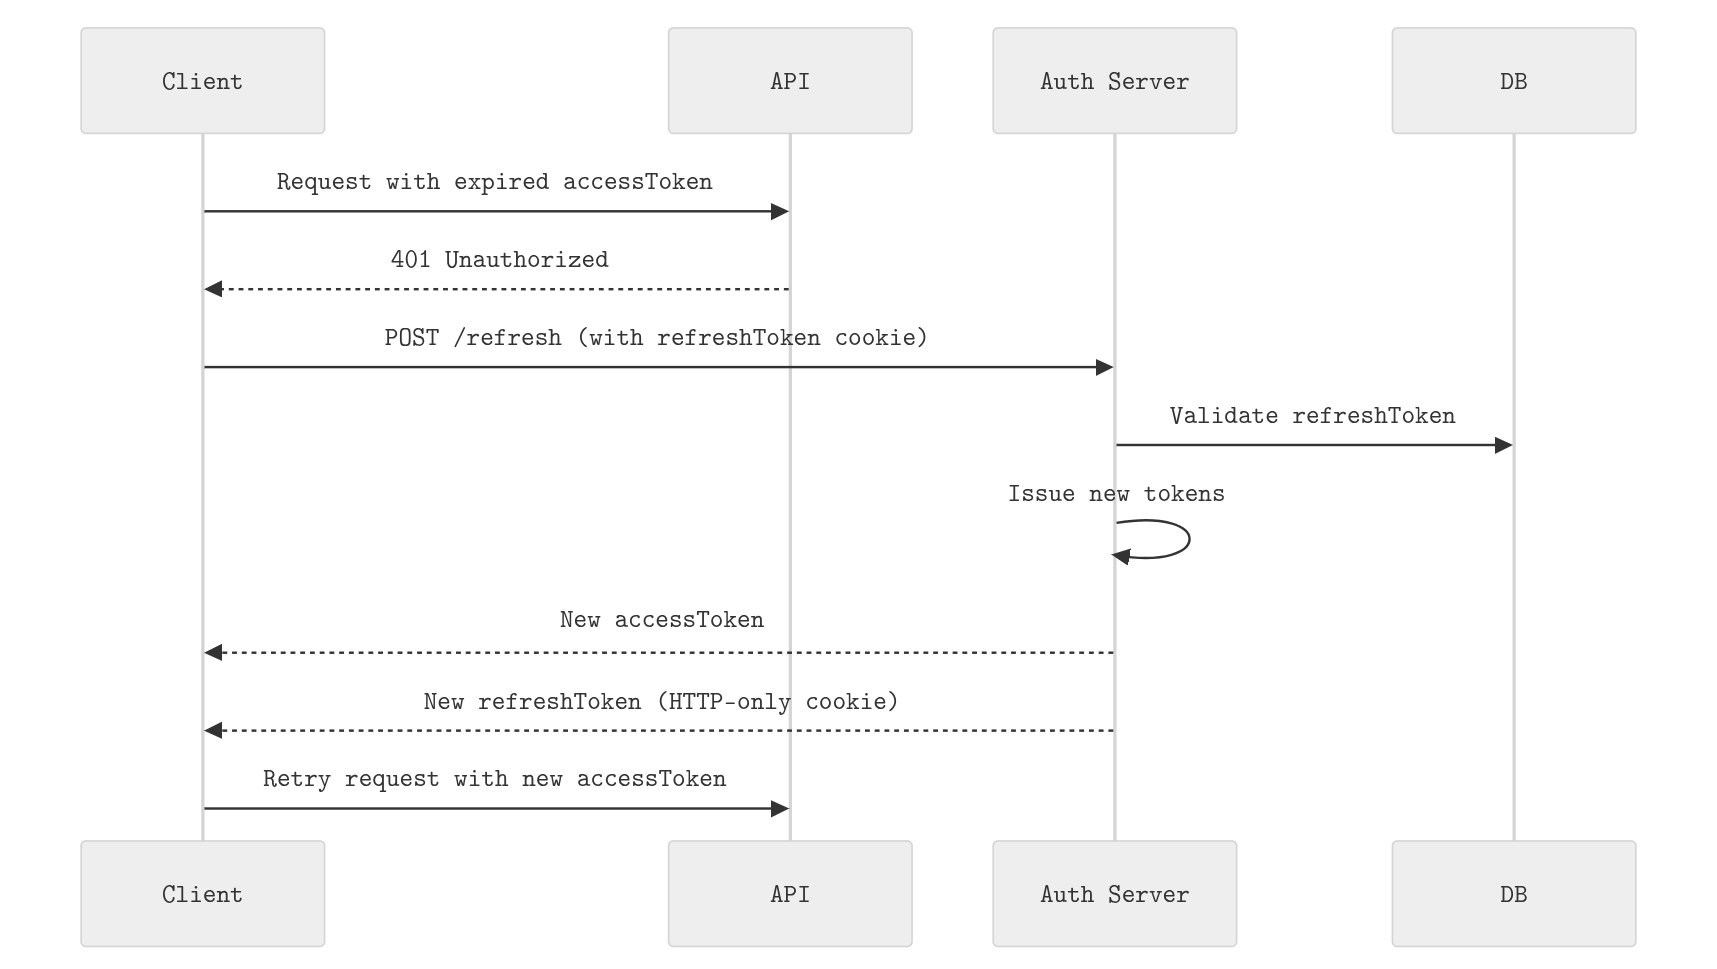
\includegraphics[width=\textwidth]{images/silent-refresh.png}
              \caption{Silent refresh flow.}
              \label{fig:silent refresh}
          \end{figure}

          Considerations

          \begin{itemize}
              \item Refresh token is never exposed to JS (\texttt{HttpOnly} cookie)

              \item Server rotates refresh tokens (invalidates old one)

              \item If refresh token is invalid/expired, force logout
          \end{itemize}
    \item Logout
          \begin{figure}[H]
              \centering
              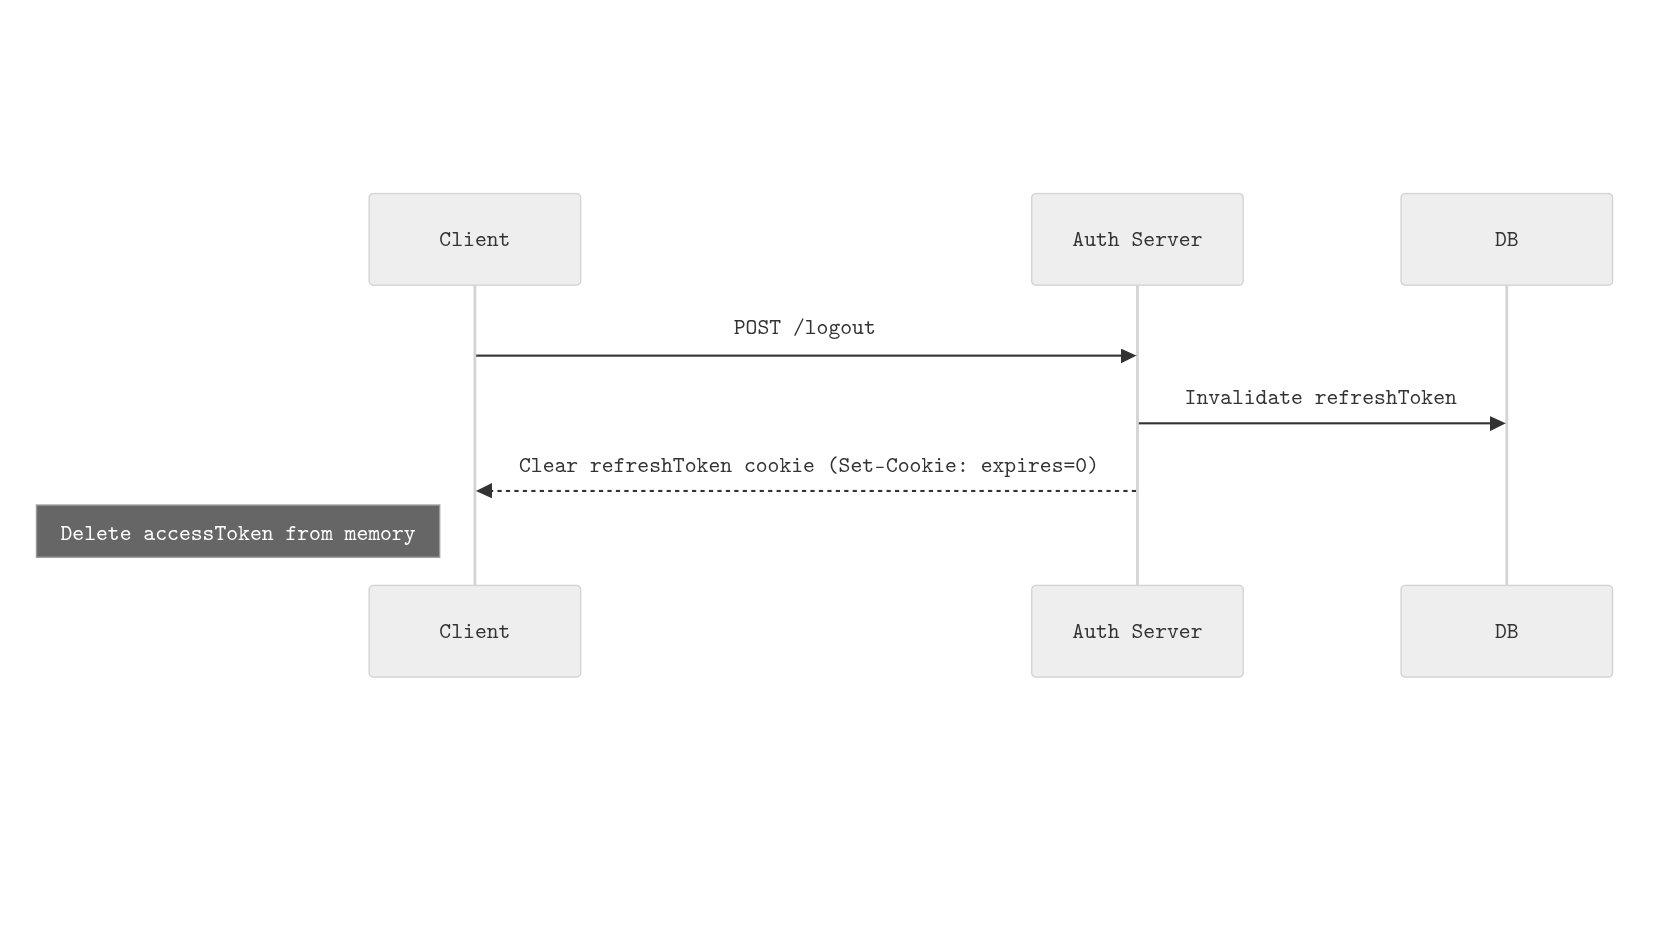
\includegraphics[width=\textwidth]{images/logout.png}
              \caption{Logout flow.}
              \label{fig:logout}
          \end{figure}

          Critical actions:

          \begin{itemize}
              \item Server adds refresh token to denylist (or deletes from DB)

              \item Client removes access token from memory

              \item Cookie is cleared via \texttt{Set-Cookie} header
          \end{itemize}
\end{enumerate}

\end{document}